\documentclass[10pt,a4paper]{article}
\usepackage[T1]{fontenc}
\usepackage{lmodern}
\usepackage[margin=20mm]{geometry}
\usepackage{amsmath,booktabs,graphicx,hyperref}
\hypersetup{colorlinks=true,linkcolor=blue,urlcolor=blue,citecolor=blue,
 pdftitle={VPIN: calculation, usage and backtests},
 pdfauthor={VPIN Python Crypto project}}
\setlength{\parindent}{0pt}
\setlength{\parskip}{5pt}
\setlength{\emergencystretch}{2em}
\graphicspath{{vpin_guide_assets/}}
\newif\ifResultsAvailable
\ResultsAvailablefalse
\newcommand{\SnapshotStart}{2020-01-01}
\newcommand{\SnapshotEnd}{2026-09-20 00:00:00 UTC}
\newcommand{\RunStatus}{data unavailable}
\newcommand{\RunError}{The requested history contains 2,347 missing one-minute candles across 15 intervals. All 15 direct API rechecks returned zero candles. Checksum-verified official archives for February 2020 and March 2023 contain the same omissions in those months. The searches were not started; no historical winner is claimed.}
\newcommand{\ReportSymbol}{BNBUSDT}
\newcommand{\DefaultBuckets}{252}
\newcommand{\DefaultWindow}{10}
\newcommand{\ADVLookback}{90}
\newcommand{\CDFLookback}{90}
\newcommand{\FeeBps}{10}
\newcommand{\SlippageBps}{2}


\begin{document}
{\LARGE\bfseries VPIN: calculation, usage and backtests\par}
{\large A practical guide to this Binance minute-data implementation\par}
\medskip
\textbf{Study snapshot:} \SnapshotStart{} to \SnapshotEnd{} (end exclusive).\\
\textbf{Status:} \RunStatus.

\section{What the indicator measures}
Volume-Synchronized Probability of Informed Trading (VPIN) summarizes absolute
buy/sell imbalance in volume-based observations. A volume clock advances when
enough trading volume has accumulated, rather than at equally spaced times.
Under the assumptions behind PIN models, persistent imbalance can be associated
with informed activity and adverse selection faced by liquidity providers
\cite{lopez,cartea}. Imbalance alone does not identify a trader's information.

This project constructs an \emph{approximation} from completed one-minute
Binance spot candles. It uses the exchange's aggregate taker-buy volume,
rather than an inferred tick rule. Minute totals do not reveal trade ordering.
High VPIN can accompany buying as well as selling; it supplies no direction.

\subsection{Data and adaptive bucket targets}
All dates and candle boundaries are UTC. For minute $m$, let $v_m$ be total
base-asset volume and $b_m$ taker-buy base volume. Sell-initiated volume is
$s_m=v_m-b_m$. For BNBUSDT these volumes are in BNB; prices are USDT per BNB.
The API fields are documented by Binance \cite{binance}. The implementation
requires finite positive prices and $0\le b_m\le v_m$.

For UTC day $d$, the target for a \emph{new} bucket is
\begin{equation}
 A_d=\frac{1}{L}\sum_{\ell=1}^{L}
       \sum_{\substack{m\text{ on complete}\\\text{UTC day }d-\ell}}v_m,
 \qquad V_d=\frac{A_d}{k},
 \label{eq:target}
\end{equation}
where $L=\texttt{adv\_lookback\_days}$ and $k$ is the target bucket count per day.
Only preceding complete days enter the average. Initial calibration rows have
no targets. A positive \texttt{bucket\_size\_base} override supplies a fixed
target and bypasses calibration.

Once a bucket starts, its target stays fixed until it fills, including across
midnight. Later buckets use the new day's target. Thus $k$ is an activity target
based on recent volume, not a guarantee of exactly $k$ observations every day.

\subsection{Filling and normalizing}
When $f$ units from a minute fill part of a bucket, assigned buys and sells
are $f\,b_m/v_m$ and $f\,s_m/v_m$. Repeat until the minute is consumed; retain
the unfinished bucket for the next minute and omit the final incomplete tail.
For the most recent $n$ full buckets,
\begin{equation}
 \mathrm{VPIN}_i=
 \frac{\sum_{j=i-n+1}^{i}|B_j-S_j|}
      {\sum_{j=i-n+1}^{i}(B_j+S_j)}.
 \label{eq:vpin}
\end{equation}
The denominator is actual rolling volume. If all bucket sizes equal $V$,
it reduces to $nV$, the fixed-volume formula in \cite[section 19.5.2, p.~292]{lopez}.
Changing daily targets is this project's extension of that setting.

\clearpage
\section{From minutes to volume buckets}
Consider these base volumes across midnight. The day change alters targets
only for buckets that have not yet started.
\begin{center}
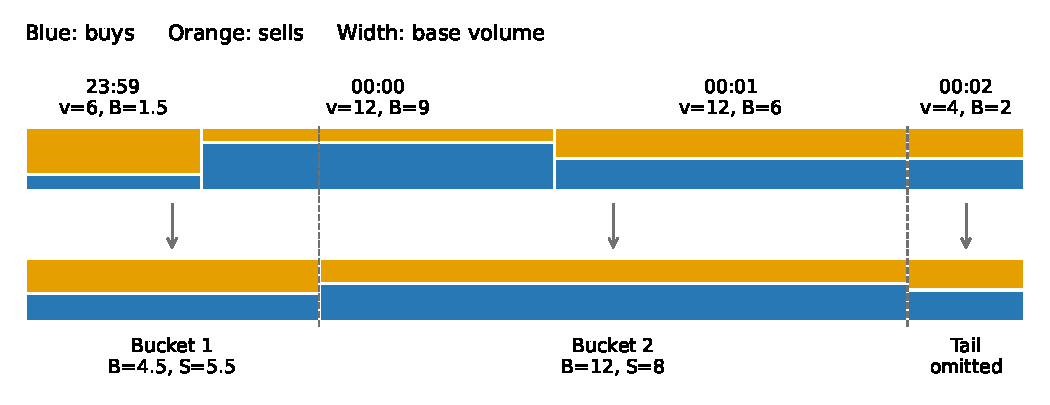
\includegraphics[width=\textwidth]{bucket_example.pdf}
\end{center}
\textbf{Worked example.} Each upper rectangle is a minute's buy/sell mixture;
vertical colors do not imply trade ordering. Dashed boundaries show where
the volume clock splits a minute. The new-bucket target changes from 10 to 20 at midnight.
Bucket 1 takes six units from 23:59 and four from 00:00:
$B_1=1.5+4(9/12)=4.5$ and $S_1=5.5$. It keeps its original target of 10.
Bucket 2 takes the remaining eight units from 00:00 and all twelve from 00:01:
$B_2=8(9/12)+6=12$ and $S_2=8$. With $n=2$,
\[
 \mathrm{VPIN}=\frac{|4.5-5.5|+|12-8|}{10+20}
             =\frac{5}{30}\simeq0.1667.
\]
The four final units remain unfinished and do not enter this estimate.

\subsection{When a value becomes usable}
A bucket's \texttt{time} is the closing timestamp of its final contributing
minute plus one millisecond. The example buckets become available at 00:01
and 00:02, respectively. Recording their starting times would introduce future
information into earlier signals.

Several buckets may complete within the same minute. Construction order is
preserved; the simulator uses the last completed bucket for that minute.
Bucket \texttt{price} is the final candle's close for plotting, not a median
trade price or a trade execution price.

\subsection{The minute-data limitation}
If a minute contains 100 buys followed by 100 sells, trade-sequenced buckets
of size 10 would be one-sided. Proportional splitting of the balanced minute
instead produces balanced buckets: VPIN 1 versus 0. Exchange aggressor totals
classify the \emph{minute}, but cannot recover its missing sequence.

\clearpage
\section{Percentiles and performance measures}
Let $\mathcal H_i$ contain preceding valid VPIN observations in the configured
$D$-day window. The current observation is excluded; ties count:
\begin{equation}
 F_i=\frac{1}{|\mathcal H_i|}
       \sum_{j\in\mathcal H_i}
       \mathbf 1\{\mathrm{VPIN}_j\le\mathrm{VPIN}_i\}.
 \label{eq:cdf}
\end{equation}
\begin{center}
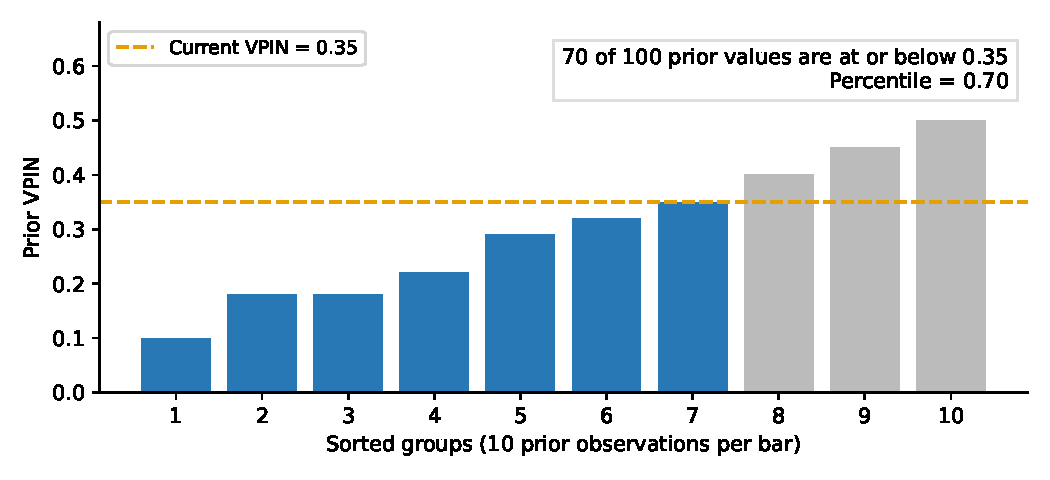
\includegraphics[width=\textwidth]{percentile_example.pdf}
\end{center}
\textbf{Reading the rank.} Each bar represents ten prior observations at the
shown value. Seven blue bars give 70 observations at or below the current
VPIN of 0.35, so $F_i=70/100=0.70$. Ties are included. The current value is
compared with the reference; it is not added to its own denominator.

The window excludes its left boundary. Earlier bucket rows with the same
availability timestamp retain their order. CDF is unavailable until $D$ days
have elapsed since the first valid VPIN and at least 100 prior values are
present. A constant reference also yields no CDF.

CDF 0.99 places the observation near the upper tail of its reference history.
It is not a 99\% crash probability or a calibrated probability that a trader
is informed.

The drawing is a constructed teaching example, not market data. It assumes
the required time history is present. It shows how the rank is calculated,
not whether a rank predicts a useful trading decision.

\subsection{Returns, drawdown, and Calmar}
Equity $E_t$ is cash plus asset quantity times the minute close. Two successive
doublings take wealth from 1 to 4: a 300\% return. A decline from 2 to 1 is
a 50\% drawdown. Including initial capital in the peak,
\[
 DD_t=100\left(\frac{E_t}{\max_{u\le t}E_u}-1\right).
\]
Over $d$ calendar days, compound annual growth rate and the selection score are
\[
 \mathrm{CAGR}=100\left[\left(\frac{E_T}{E_0}\right)^{365.25/d}-1\right],
 \qquad \mathrm{Calmar}=\frac{\mathrm{CAGR}}{|\min_t DD_t|}.
\]
Costs enter equity before these metrics are calculated. Zero drawdown or
nonfinite annualization makes a candidate ineligible.

\clearpage
\section{Basic strategy and usage}
This is a long-or-cash risk-exit experiment, not a market-making implementation.
\begin{center}
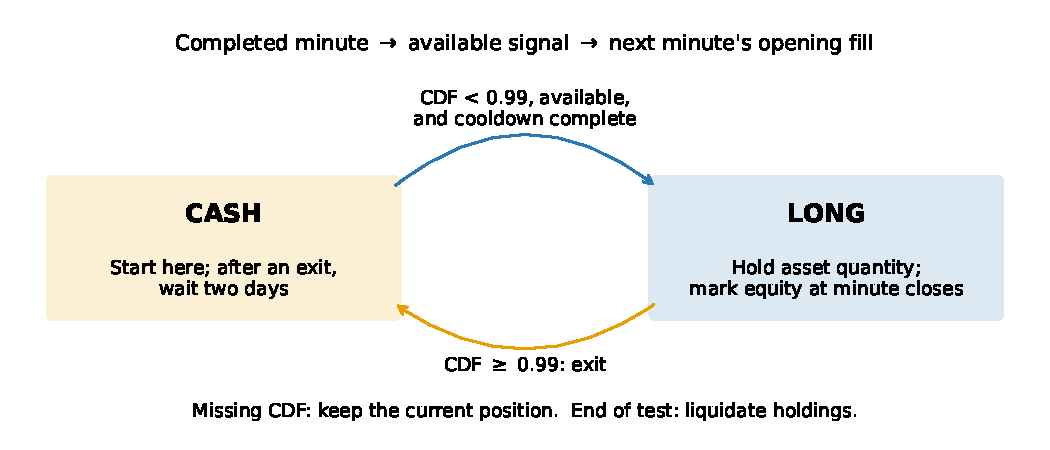
\includegraphics[width=\textwidth]{strategy_flow.pdf}
\end{center}
Start each scoring interval with unit cash. The two-day cooldown starts at
the actual exit, not when a bucket begins. At the end, remaining holdings
are sold at the final candle close; this liquidation is not a signal exit.
A signal formed when a candle finishes can first act at the next candle's
open. Exit takes precedence over re-entry, preventing a same-time round trip.

\subsection{Configuration}
\begin{center}\small
\begin{tabular}{ll}
\toprule
Setting & Study configuration\\
\midrule
Symbol / requested history start & \ReportSymbol{} / \SnapshotStart\\
Baseline buckets/day / VPIN window & \DefaultBuckets{} / \DefaultWindow{}\\
ADV / CDF lookback & \ADVLookback{} / \CDFLookback{} days\\
Fixed bucket override & None: adaptive targets\\
Fee / slippage per side & \FeeBps{} / \SlippageBps{} basis points\\
Exit threshold / cooldown & 0.99 / 2 days\\
\bottomrule
\end{tabular}
\end{center}
The study does not silently change application defaults. The baseline 252/10
settings are provisional. Costs are adjustable assumptions, not the user's
actual exchange fee tier. Cash earns no interest.

\subsection{Commands}
Use Python 3.10+ from the project root:
\begin{verbatim}
pip install pandas numpy aiohttp matplotlib pyarrow tqdm optuna
python -m unittest -q test_vpin
python market_data.py
python vpin_calculator.py
python vpin_backtest.py
python vpin_optuna_optimize.py
\end{verbatim}
Edit \texttt{config.json} for the instrument and a valid data interval.
The downloader repairs missing ranges and refreshes overlapping closed
candles. Unresolved gaps stop analysis. Old timezone-naive caches are rebuilt
because historically truncated candles cannot be identified reliably.

\clearpage
\section{Search design and empirical results}
\subsection{Training and held-out evaluation}
Both methods use the same data, warmup, simulator, costs, and scoring dates.
The common warmup uses 20 buckets/day and a 350-bucket window, or more
demanding configured values. Candidates without usable history at the shared
start are rejected.

After warmup, the first 80\% of elapsed time is training and the last 20\%
is held out. The protocol requests 143 grid combinations and 100 Optuna TPE trials
(seed 42, 20 startup trials), searching 20--350 buckets/day and windows
10--350. Eligibility requires at least 30 training signal exits and finite
Calmar. Only training Calmar selects a winner.

The held-out comparison includes each method's winner and the current
252/10 setting, deduplicating identical configurations. Each starts with fresh
cash while retaining preceding indicator history. Buy-and-hold uses identical
dates and entry/terminal cost assumptions. A poor test result does not cause
another configuration to be selected.

\ifResultsAvailable
\textbf{Validated snapshot:} \DataRows{} candles.
Training begins \TrainingStart{} UTC; the held-out interval begins
\SplitTime{} UTC and ends at \SnapshotEnd.

\textbf{Eligibility:} \GridEligible{} grid rows and \OptunaEligible{} Optuna
trials qualified. The table below deduplicates repeated configurations.
\WinnerText

\subsection{Top five distinct training configurations}
\begin{center}\small\TrainingTable\end{center}
Here $k$ is buckets/day, $n$ is the rolling bucket count, and DD is negative
percentage drawdown. Ranking uses training Calmar only.

\subsection{Frozen held-out comparison}
\begin{center}\small\HeldOutTable\end{center}
Exit counts exclude terminal liquidation. Buy-and-hold has no signal exits.
\emph{Best} means best training Calmar among the searched configurations,
not a guarantee of future performance or a global optimum.
\else
\subsection{Results unavailable under the requested constraints}
\textbf{Study status: \RunStatus.} \RunError

No winning configuration or performance table is asserted. Old avoided-
drawdown statistics and synthetic tests are not empirical substitutes.
Coverage must pass before either full search supplies results. Any change
to the study interval must be explicit and recorded.
\fi

\subsection{Interpreting results}
Selling during strong buying can miss upside. Judge cost-adjusted test return
and drawdown together with the benchmark. A brief dip while in cash does not
prove that an exit was beneficial; the former cumulative avoided-drawdown
score was removed for this reason.

Minute-close equity omits intraminute extremes. Fixed-slippage opening fills
do not model spread dynamics, order-book depth, impact, latency, or trading
halts. Repeatedly tuning after inspecting the test period would consume its
independence. No uncertainty interval or prediction accuracy is established
by Calmar alone.

\ifResultsAvailable
\clearpage
\section{Held-out equity and drawdown}
\begin{center}
\includegraphics[width=\textwidth]{equity_drawdown.pdf}
\end{center}
\textbf{Historical comparison.} Wealth and drawdown for the training-selected configurations,
current defaults, and buy-and-hold. Identical configurations share a curve.
The plot uses daily closing wealth and each day's worst minute-close
drawdown; reported metrics use every minute.

Flat strategy segments indicate cash exposure. Differences from buy-and-hold
include avoided losses, missed gains, and the costs of repeated trading.
This comparison concerns one spot instrument, one chronological split, and
the stated cost assumptions.

\clearpage
\section{Reading the indicator example}
\begin{center}
\includegraphics[width=0.88\textwidth]{indicator_example.pdf}
\end{center}
\textbf{Historical indicator example.} Predetermined final 14 days of the snapshot, using
configuration \IllustrationConfig. Price is the close of the candle that
completed each bucket. Shading marks CDF at least 0.99; it does not label a
subsequently observed crash. The illustrated configuration is the training
winner, or the explicitly identified default if none qualified.
\fi

\clearpage
\section{Book context, verification, and reproduction}
These are original summaries of relevant ideas, not reproductions of the
source books.

\textbf{PIN and volume clocks.}
L\'opez de Prado \cite[section 19.5.2, p.~292]{lopez} relates normalized
imbalance to PIN under arrival-model assumptions. The fixed-volume algebra
supports the special case of Eq.~\eqref{eq:vpin}; the discussion also records
conflicting findings about volatility prediction. Correct arithmetic alone
does not establish forecasting value.

\textbf{Calibration is a separate result.}
The futures study summarized in \cite[section 22.6.5, pp.~346--347]{lopez}
covers approximately 100 contracts over 67 months. Its example settings
include 200 buckets/day, 30 \emph{bars per bucket}, one-day VPIN support,
0.1-day events, median trade prices, Student-$t$ bulk classification ($\nu=0.1$), and a
0.99 CDF threshold. The underlying report separates bar construction from
the number of buckets used in VPIN \cite{wu}. Thirty bars per bucket is
not a 30-bucket rolling window; this calibration does not validate the
project's adaptive minute-based crypto settings. That study evaluates volatility
events rather than this long/cash strategy's returns.

\textbf{Other context.}
Jansen \cite[pp.~38--39]{jansen} explains volume bars, illustrates timestamps
at the last constituent trade, and discusses dollar bars when price changes
affect comparisons. Cartea, Jaimungal, and Penalva \cite[p.~70]{cartea}
discuss PIN alongside information asymmetry and market quality. Neither
supplied a separate VPIN calibration used here. The scanned Cartea volume
was inspected through its index and related pages, not exhaustive OCR.

Section 19.7 of \cite[pp.~295--296]{lopez} concerns predictive losses and
microstructural information, not this empirical CDF. A high/low midpoint is
not a median trade price. With supplied aggressor totals, the project's
plotted bucket prices do not enter Eq.~\eqref{eq:vpin}.

\subsection{Reproduction}
The manifest records configuration, source/data hashes, versions, and coverage
outcome. A completed study also records scoring dates and seed, with full
training trials and selected held-out metrics in CSV files. Rebuilding generates
tables from that evidence and verifies its hashes without rerunning optimization.
Text fingerprints normalize CRLF line endings to LF; binary fingerprints are byte-exact.
Rebuild or refresh with:
\begin{verbatim}
python docs/build_vpin_guide.py
python docs/build_vpin_guide.py --run-backtests
\end{verbatim}
Use \texttt{--start-date YYYY-MM-DD} and \texttt{--end-date YYYY-MM-DD}
with the second command to set an explicit study interval (end exclusive)
without changing \texttt{config.json}. Tests cover independent arithmetic, data boundaries,
causality, execution, costs, and selection. Grid/Optuna agreement checks their
integration rather than independently proving the numerical model.

\begin{thebibliography}{9}\small
\bibitem{lopez} M.~L\'opez de Prado. \emph{Advances in Financial Machine Learning}.
Wiley, 2018. Sections 19.5.2, 19.7, and 22.6.5.
\bibitem{jansen} S.~Jansen. \emph{Machine Learning for Algorithmic Trading},
2nd ed. Packt, 2020, pp.~38--39.
\bibitem{cartea} \'A.~Cartea, S.~Jaimungal, and J.~Penalva.
\emph{Algorithmic and High-Frequency Trading}. Cambridge University Press, 2015, p.~70.
\bibitem{wu} K.~Wu, E.~W.~Bethel, M.~Gu, D.~Leinweber, and O.~R\"ubel.
\emph{A Big Data Approach to Analyzing Market Volatility}. LBNL-6382E, 2013.
\href{https://sdm.lbl.gov/~kewu/ps/LBNL-6382E.pdf}{Public technical report}.
\bibitem{binance} Binance. \emph{Spot REST API: Market data endpoints}.
\href{https://developers.binance.com/docs/binance-spot-api-docs/rest-api/market-data-endpoints}{Official kline documentation}.
Accessed 20 September 2026.
\end{thebibliography}
\end{document}
